% =====================================================================================================
%
%  ABSTRACT
%
% =====================================================================================================
\begingroup
\renewcommand{\cleardoublepage}{}
\renewcommand{\clearpage}{}
\chapter*{Abstract}\label{chap:abstract}
\addcontentsline{toc}{chapter}{Abstract}
\renewcommand{\chapter}[2]{}%q

\lettrineabstract{Lorem ipsum dolor sit amet, consectetur adipiscing elit. Fusce maximus nisi ligula. Morbi laoreet ex ligula, vitae lobortis purus mattis vel. Vestibulum ante ipsum primis in faucibus orci luctus et ultrices posuere cubilia Curae; Donec ac metus ut turpis mollis placerat et nec enim. Duis tristique nibh maximus faucibus facilisis. Praesent in consequat leo. Maecenas condimentum ex rhoncus, elementum diam vel, malesuada ante.}

%----------------------------------------------------------------------------------------
%	ARTICLE CONTENTS
%----------------------------------------------------------------------------------------

\section{Introduction}
\label{sec:Abstract_Introduction}

This sentence requires citation \cite{Devlin2019}. This sentence requires multiple citations to imply that it is better supported \citep{Kim2016,Rajpurkar2016}. Finally, when conducting an appeal to authority, it can be useful to cite a reference in-text, much like \citep{Tenney2020} do quite a bit. Oh, and make sure to check out the bear in Figure \ref{fig:Abstract_FigureExample}.

\begin{figure}[ht]
	\begin{align}
	A = 
	\begin{bmatrix}
	A_{11} & A_{21} & A_{31} \\
	A_{21} & A_{22} & A_{32}
	\end{bmatrix}
	\end{align}
	\caption{Figure Example}
	\label{fig:Abstract_FigureExample}
\end{figure}

\subsection{NLP Tasks}
\label{sec:Abstract_Introduction_NLP_Tasks}

Lorem ipsum dolor sit amet, consectetur adipiscing elit. Fusce maximus nisi ligula. Morbi laoreet ex ligula, vitae lobortis purus mattis vel. Vestibulum ante ipsum primis in faucibus orci luctus et ultrices posuere cubilia Curae; Donec ac metus ut turpis mollis placerat et nec enim. Duis tristique nibh maximus faucibus facilisis. Praesent in consequat leo. Maecenas condimentum ex rhoncus, elementum diam vel, malesuada ante. Fusce pulvinar, mauris pretium placerat venenatis, lectus ex tempus lacus, id suscipit libero lorem eu augue. Interdum et malesuada fames ac ante ipsum primis in faucibus. \\

Donec nec nibh sagittis, finibus mauris quis, laoreet augue. Maecenas aliquam sem nunc, vel semper urna hendrerit nec. Pellentesque habitant morbi tristique senectus et netus et malesuada fames ac turpis egestas. Maecenas pellentesque dolor lacus, sit amet pretium felis vestibulum finibus. Duis tincidunt sapien faucibus nisi vehicula tincidunt. Donec euismod suscipit ligula a tempor. Aenean a nulla sit amet magna ullamcorper condimentum. Fusce eu velit vitae libero varius condimentum at sed dui. \\

\begin{figure}[!ht]
	\centering
	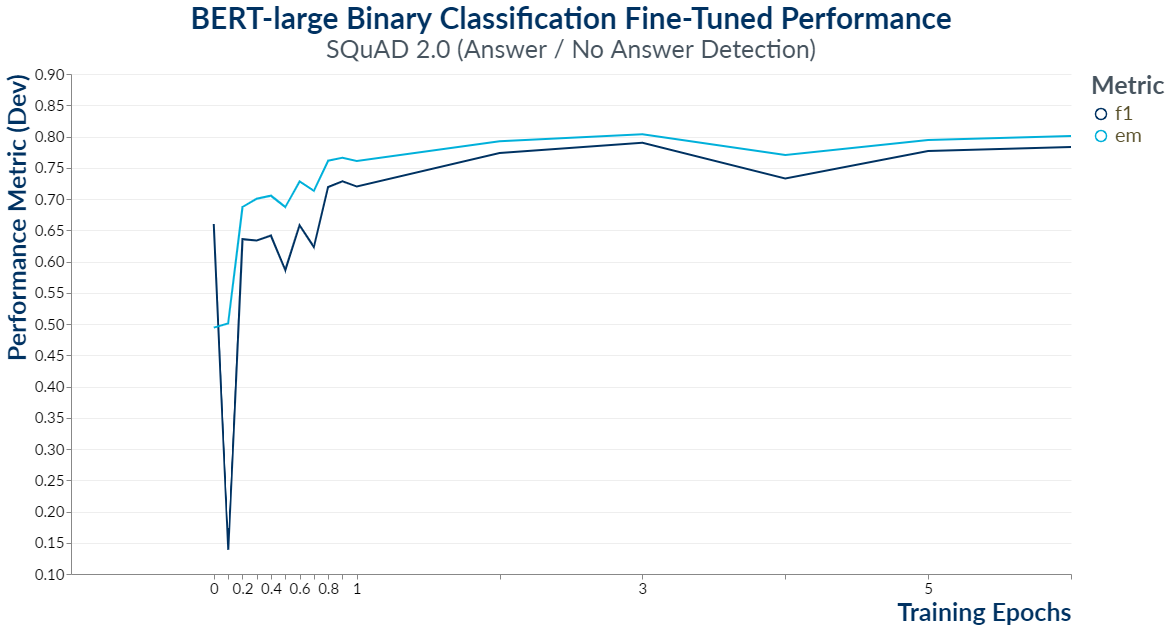
\includegraphics[width=\linewidth,height=2in]{BinaryClassification_BERT_Training_Performance_plot.png}
	\caption{Image Figure Example}
	\label{fig:Abstract_ImageFigureExample}
\end{figure}

%----------------------------------------------------------------------------------------
\endgroup